\documentclass[oneside, 11pt]{book}
\usepackage[titletoc]{appendix}
\usepackage{geometry}
\usepackage{natbib}
\usepackage{epsfig}
%\usepackage{hyperref}
\usepackage{upgreek}
\usepackage{bbold}
\usepackage[english]{babel}
\usepackage[applemac]{inputenc}
\usepackage{setspace}
\usepackage{caption}
\usepackage{amsthm}
\usepackage{float}
\usepackage{placeins}
\usepackage{natbib}
\usepackage{amsmath,amsfonts,amsthm,amssymb}
\usepackage{url}
\usepackage{multirow}
\usepackage{subfigure}
\usepackage{algorithm}
\usepackage[noend]{algpseudocode}
\newtheorem{mydef}{Definition}
\onehalfspacing
\makeatletter
\def\url@leostyle{%
  \@ifundefined{selectfont}{\def\UrlFont{\sf}}{\def\UrlFont{\small\ttfamily}}}
\makeatother
\geometry{a4paper,left=24mm,right=24mm, top=33mm, bottom=3.1cm}
\urlstyle{leo}
\usepackage{fancyhdr}
\pagestyle{fancy}
\fancyhf{}
\fancyhead[C]{Active Sampling as Bayesian Quadrature}
\fancyfoot[C]{ \thepage}

\begin{document}


\newcommand{\hmwkCourse}{MSc Cognitive and Decision Sciences\vspace{18mm}}
\newcommand{\hmwkTitle}{{\bf Active Sampling as Bayesian Quadrature} \vspace{18mm} \\ 
Master of Science -Thesis}
\newcommand{\hmwkSubTitle}{} % No subtitle, so this will be excluded
\newcommand{\hmwkDueDate}{\today}
\newcommand{\hmwkClassInstructor}{}
\newcommand{\hmwkAuthorName}{Christoph Niemeyer}
\newcommand{\LastPage}{TBA}

\begin{titlepage}
\vspace{20mm}
\begin{center}
\vspace{150mm}
\LARGE{ UNIVERSITY COLLEGE LONDON \\ \hmwkCourse \\[6.5cm]

\includegraphics[width=4cm]{ucl.jpg}\\
\vspace{-110mm}
 {\hmwkTitle}  \\}
\vspace{80mm}
\Large Submission for Candidate:\\
Christoph Niemeyer\\
Department of Experimental Psychology
\\
\Large \today\vspace{28mm} \\ 
\begin{tabular}{ll}
Primary Supervisor:&Eric Schulz\\
Second Grader: &Maarten Speekenbrink
\end{tabular}
\end{center}
\end{titlepage}
\vspace*{1cm}
\begin{center}
\textbf{{\LARGE Declaration of Authorship:}}\\
\end{center}
\vspace{1cm}
\begin{enumerate}
\item I am aware of the University's disciplinary regulations concerning conduct in examinations and, in particular, of the regulations on plagiarism.
\item The thesis work I am submitting is entirely my own work except where otherwise indicated.
\item This thesis has not been submitted, either wholly or substantially, for another degree of this University, or for a degree at any other institution.
\item I have clearly signaled the presence of quoted or paraphrased material and referenced all sources.
\item I have acknowledged appropriately any assistance I have received in addition to that provided by my supervisor.
\item I have not sought assistance from any professional agency. 
\end{enumerate}
\vspace{2cm}
\begin{center}
Christoph Niemeyer, \today
\end{center}
\newpage
\begin{center}
\textbf{{\LARGE Abstract:}}\\
\end{center}
How can and should an agent actively learn about probability distributions? Psychological theories involving sampling are vast, but currently there is no real theory about how humans actively acquire knowledge about explicit probability distributions. The thesis at hand therefore tries to develop a theory of active sampling based on \emph{Gaussian Processes Quadrature}, a non-parametric class of density estimation.\\
The thesis will first summarize current psychological theories about human sampling and then introduce Gaussian Processes as an approach to Quadrature. It will be shown how Gaussian processes can be used to explore any probability distribution.\\
Multiple different sampling metaphors will be stated and all of them will be tested at how well they describe participants' active sampling behavior within a simple active density exploration task. Overall the Gaussian Process-based Quadrature approach will be shown to describe participants' behavior best.\\
The thesis will continue and define a rather new niche to compare different sampling models based on how well they can predict human active sampling behavior. Potential consequences and future experiments based on this assay will be examined.\\
Limitations and connections to related research questions will be discussed.\bigskip\\
\begin{center}
\textbf{KEYWORDS:} Active Sampling, Bayesian Quadrature, Gaussian Processes
\end{center}
\newpage
\vspace*{1cm}
\begin{center}
\textbf{{\LARGE Acknowledgements:}}\\
\end{center}
Thanks to Eric Schulz, you're a wonderful human being! Also, my parents are nice, too.
\newpage
%%%%%%%%%%%%%%%%%%%%%%%%%%%%%%%%%%%%%%%%%%%%%%%%%%%%%%%%%%%%%%%%%%%%%%%%%%%%%%%%%%%
\vspace*{10cm}
\begin{center}
\textbf{\Large{``I love the creativeness of raw sampling.''}} (Moreno about Depeche Mode)
\end{center}
\newpage
%%%%%%%%%%%%%%%%%%%%%%%%%%%%%%%%%%%%%%%%%%%%%%%%%%%%%%%%%%%%%%%%%%%%%%%%%%%%%%%%%%%
\tableofcontents
\newpage
%%%%%%%%%%%%%%%%%%%%%%%%%%%%%%%%%%%%%%%%%%%%%%%%%%%%%%%%%%%%%%%%%%%%%%%%%%%%%%%%%%%
\chapter{Introduction}
Many psychological theories are based on strong sampling assumptions, be it either as a metaphor for memory search or as a description for decision making. However, all of those theories are based on very simplistic sampling assumptions, most commonly that the cognitive agent performs, either explicitly or implicitly, a random walk over the population set sampled from. However, a random walk algorithms can be both very inefficient and implausible. Here, we develop a theory of active human sampling when the task is to judge about probabilities of events after a prior explicit sampling period. We argue that humans are not at always sampling completely at random, but rather makes sense of their environment by using highly adaptive and cleverly designed sampling mechanisms, derived from a powerful Bayesian quadrature algorithm.\medskip\\
Chapter \S2 draws out a vision of a Bayesian Cognitivism and defines quadrature as an essential part of it. Chapter \S3 sets up the problem of quadrature and describes different sampling algorithms that have been proposed in the psychological literature as well as in statistical research. Chapter \S4, the methods section, sets up the design of the experiment and describes the participants in more detail. Chapter \S5 illustrates the results of the experiment and Chapter \S6 discusses potential problems, shortcomings, and future steps. Chapter \S7 will conclude the thesis by a call for more elaborate comparisons between different proposed sampling schemes.

%%%%%%%%%%%%%%%%%%%%%%%%%%%%%%%%%%%%%%%%%%%%%%%%%%%%%%%%%%%%%%%%%%%%%%%%%%%%%%%%%%%%%%%%%%%%%%%
\chapter{Bayesian Cognitivism}
\emph{This chapter will briefly describe a vision of Bayesian Cognitivism. Bayesian Cognitivism seeks out to model an intelligent system based on non-parametric Bayesian approaches that quantify uncertainty for each part. Quadrature is an important part thereof.}
\section{Different parts of an intelligent system}
\begin{figure}
\caption{Bayesian Cognitivism based on non-parametric models.}
\label{dense}
  \centering
    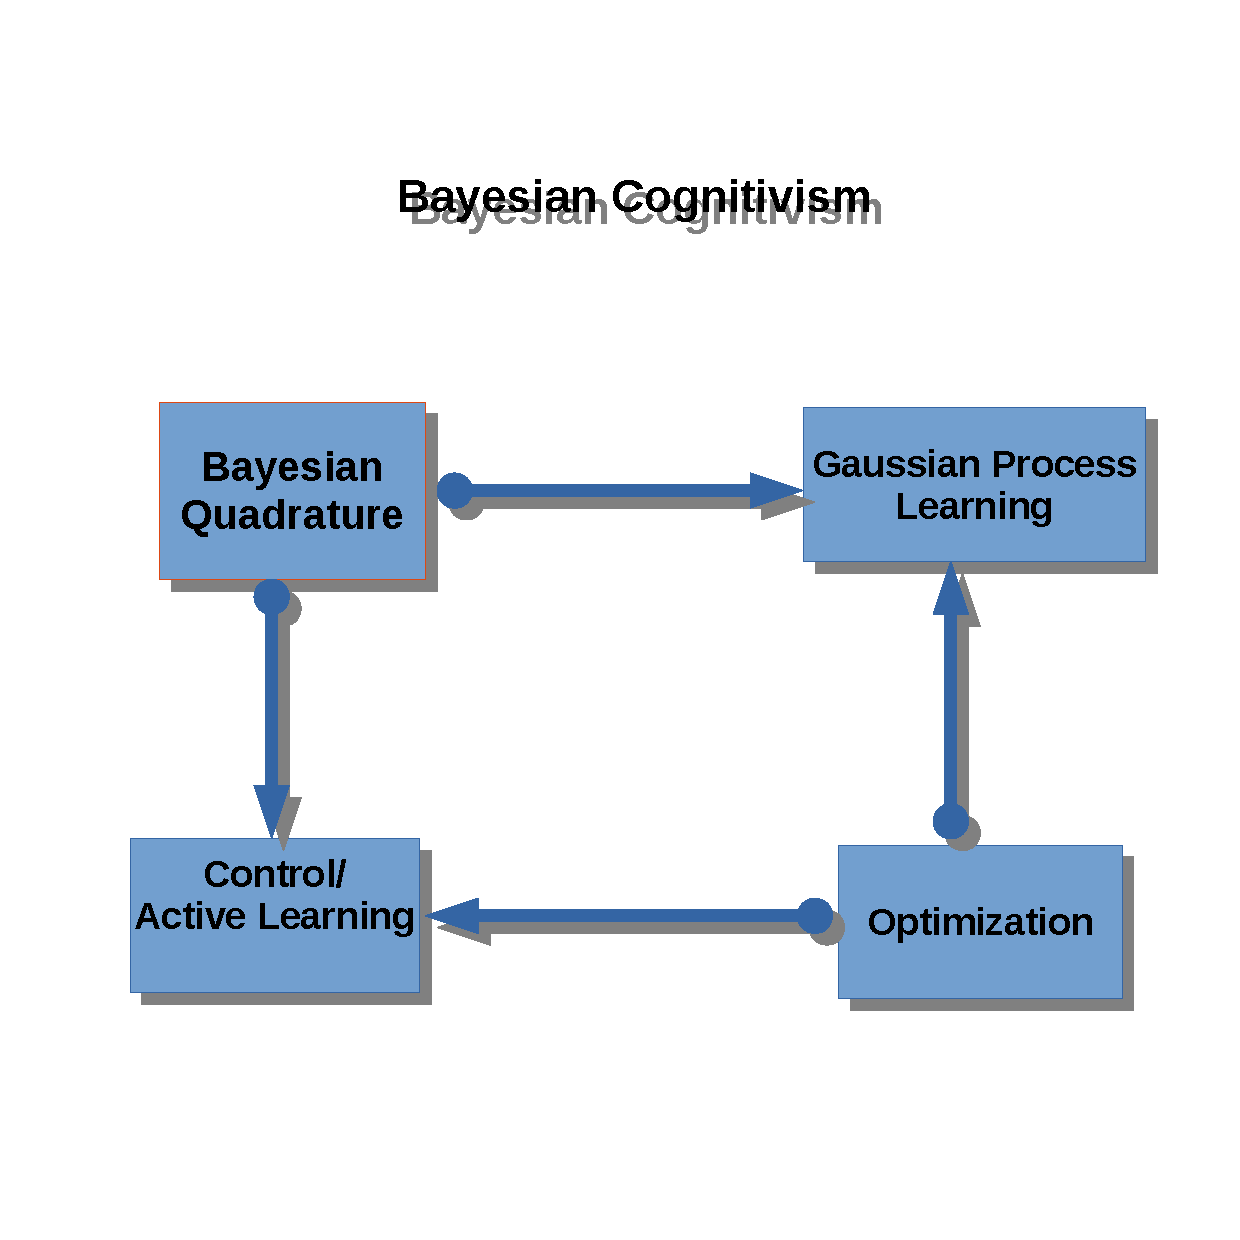
\includegraphics[scale=0.6]{bayescog.pdf}
 \label{denseb}
\end{figure}
Don't forget to cite your supervisor \citep{schulz2015learning}.
\section{Quadrature}
What is it? And why should the reader care about it?

%%%%%%%%%%%%%%%%%%%%%%%%%%%%%%%%%%%%%%%%%%%%%%%%%%%%%%%%%%%%%%%%%%%%%%%%%%%%%%%%%%%%%%%%%%%%%%%
\chapter{Quadrature}
\emph{This chapter will set up the problem of Quadrature and describe different approaches to solve this problem actively.}

\section{The problem: expectations over functions}
\begin{align}
Z=\int f(x)p(x) dx
\end{align}
\section{Active Sampling Approaches}
\subsection{Random Walk}
\subsection{Metropolis}
\begin{align}
\hat{Z}=\frac{1}{N}\sum_{i=1}^nf(x)
\end{align}
\subsection{Whatever else you like}
\subsection{Bayesian Quadrature}

%%%%%%%%%%%%%%%%%%%%%%%%%%%%%%%%%%%%%%%%%%%%%%%%%%%%%%%%%%%%%%%%%%%%%%%%%%%%%%%%%%%%%%%%%%%%%%%

\chapter{Methods}
\emph{This chapter will provide a detailed description of the used design and recruited participants.}
\section{Design}
\section{Participants}

%%%%%%%%%%%%%%%%%%%%%%%%%%%%%%%%%%%%%%%%%%%%%%%%%%%%%%%%%%%%%%%%%%%%%%%%%%%%%%%%%%%%%%%%%%%%%%%
\chapter{Results}
\emph{This chapter will show the results of the experiment both in raw and modeled format.}
\section{Raw results}
\section{Modeling results}
%%%%%%%%%%%%%%%%%%%%%%%%%%%%%%%%%%%%%%%%%%%%%%%%%%%%%%%%%%%%%%%%%%%%%%%%%%%%%%%%%%%%%%%%%%%%%%%
\chapter{Discussion}
\emph{This chapter will discuss the results and explain why the Bayesian Quadrature method outperformed the other methods.}

%%%%%%%%%%%%%%%%%%%%%%%%%%%%%%%%%%%%%%%%%%%%%%%%%%%%%%%%%%%%%%%%%%%%%%%%%%%%%%%%%%%%%%%%%%%%%%%
\chapter{Conclusion}
\emph{This chapter will conclude the thesis by calling for more elaborate assessments of human active sampling.}

\bibliographystyle{apa-good}
{\footnotesize\bibliography{Bibo}}


%%%%%%%%%%%%%%%%%%%%%%%%%%%%%%%%%%%%%%%%%%%%%%%%%%%%%%%%%%%%%%%%%%%%%%%%%%%%%%%%%%%%%%%%%%%%%%%
\end{document}